
\documentclass[review]{elsarticle}

\usepackage{lineno,hyperref}
\usepackage[mathletters]{ucs}
\usepackage[utf8x]{inputenc}
\usepackage[linesnumbered, ruled, vlined]{algorithm2e}
\usepackage{natbib}
\usepackage{supertabular}
\usepackage{fancybox}
\usepackage{acronym}
\usepackage{array}
\usepackage{booktabs}
\usepackage{graphicx}
\usepackage{rotating}
\usepackage{tabularx}
\usepackage{multirow}
\usepackage{hhline}
\usepackage{setspace}
\usepackage{placeins}
\usepackage{longtable}
\usepackage{mathtools}
\usepackage{listings}
\usepackage{epstopdf}
\usepackage{subfigure}
\usepackage{courier}
\usepackage{amsfonts}
\usepackage{morefloats}
\usepackage{lipsum}
\usepackage{amsthm,amsmath}

% table
\usepackage{color, colortbl}
\definecolor{Gray}{gray}{0.9}

% appendix
\usepackage[titletoc,title]{appendix}
\usepackage{hyperref}
\usepackage{cleveref}

\modulolinenumbers[5]

\journal{Journal of Network and Computer Applications}

%%%%%%%%%%%%%%%%%%%%%%%
%% Elsevier bibliography styles
%%%%%%%%%%%%%%%%%%%%%%%
%% To change the style, put a % in front of the second line of the current style and
%% remove the % from the second line of the style you would like to use.
%%%%%%%%%%%%%%%%%%%%%%%

%% Numbered
%\bibliographystyle{model1-num-names}

%% Numbered without titles
%\bibliographystyle{model1a-num-names}

%% Harvard
%\bibliographystyle{model2-names.bst}\biboptions{authoryear}

%% Vancouver numbered
%\usepackage{numcompress}\bibliographystyle{model3-num-names}

%% Vancouver name/year
%\usepackage{numcompress}\bibliographystyle{model4-names}\biboptions{authoryear}

%% APA style
%\bibliographystyle{model5-names}\biboptions{authoryear}

%% AMA style
%\usepackage{numcompress}\bibliographystyle{model6-num-names}

%% `Elsevier LaTeX' style
\bibliographystyle{elsarticle-num}
%%%%%%%%%%%%%%%%%%%%%%%

\begin{document}

\begin{frontmatter}

\title{Higher Moments Distances from Robust Subspace for Botnet Detection}

%% Group authors per affiliation:
\author[unbaddress]{Thiago P. B. Vieira}
\author[unbaddress]{Eduardo Said Calil Vilaça}
\author[unbaddress,Ilmenauaddress,Fraunhoferaddress]{João Paulo C. L. da Costa}
\author[unbaddress]{Rafael T. de Sousa Júnior}

\address[unbaddress]{Department of Electrical Engineering, University of Brasilia (UnB), 70910-900, Brasília-DF, Brazil}
\address[Ilmenauaddress]{Institute for Information Technology, Ilmenau University of Technology, Ilmenau, Germany}
\address[Fraunhoferaddress]{Fraunhofer Institute for Integrated Circuits IIS, Erlangen, Germany}


\begin{abstract}
Distributed attacks organized by botnet has increasing and demanding the development of counter measures in order to detect and avoid botnet's attacks. This paper proposes an approach based on higher moments distances from robust subspace for botnet detection, applied to new features generated by flow aggretation, in a semi-supervisioned fashion and without the computational cost of new robust subspace learning for new observations. Experimental results reveal that the proposed approach outerperforms widely adoted algorithms and a method based on robust estimates and robust skewness for network anomaly detection.
\end{abstract}

\begin{keyword}
Network Anomaly Detection \sep Botnet Detection \sep Higher Moments \sep Robust Principal Component Analysis \sep Mahalanobis Distance
\end{keyword}

\end{frontmatter}

\linenumbers

%%%%%%%%%%%%%%%%%%%%%%%%%%%%%%%%%%%%%%%%%%%%%%%%%%%%%%%%%%%%%%%%%%%%%%%%%%%%%%%%%%%%%%%%%%%%%%%%%%%%%%%%%%%%%%%%%%%%%%%%%%%%%%%%%%%%%%%%%%%%%%%%%%%%%%%%%%%%%%%%%%%%%%%%%%%%%%%%%%%%%%%%%%%%%%%%%%%%%%%%%%%%%%%%%%%%%%%%%%%%
\section{Introduction}
\label{sec:introduction}

Anomaly detection can be defined as the identification of rare and suspicions events by differing the normal or majority of the data. Anomalies are also referred to as outliers, novelties, noise or deviations, and can be related to network attacks, frauds or defects \cite{bhuyan2014network,ahmed2016survey}. Anomalies can be hard to identify and separate from normal data due to the rare occurrencies of anomalies in comparison to normal events, therefore anomaly detection algorithms have to be high discriminative, robust to contamination and able to deal with the imbalanced data problem \cite{he2008learning}.

Several efforts and reasearches aim to avoid network attacks based on known attackers, fingerprints or other patterns. However, distributed attacks organized by botnet has increasing and demanding the development of counter measures in order to detect and avoid unkown attacks or even to deal with adversarial changes on behavior, location and other patterns, in order to avoid detection by behavioral or pattern based detecion systems \cite{gu2008botminer, garcia2014empirical,khattak2015botflex,acarali2016survey,wang2017botnet,Wang2018ddosbotnetssurvey}. To face this problem, it is possible to adopt unsupervised or semi-pervised approaches for network anomaly detection, where it is not necessary known anomalies for trannning models \cite{moustafa2019holistic}.

Network anomaly detection problems are usually characterized by skewed and imbalanced data \cite{Phua2004minority,he2008learning,benson2010network}. Learning algorithms for imbalanced data has been a challenging research topic, considering that the fundamental issue with the imbalanced learning problem is the ability of imbalanced data to significantly compromise the performance of most standard learning algorithms \cite{he2008learning}. Some techniques can make the data discriminative for better results on imbalanced data: Data engineering (i.e. sampling \cite{he2008learning,gu2008botminer}, aggregation \cite{lakhina2005mining,gu2008botminer,callegari2011novel, garcia2014empirical, acarali2016survey}); Feature extraction (i.e. decomposition \cite{vaswani2018robust}, robust estimates \cite{zhou2017anomaly}). 

% He and Garcia \cite{he2008learning} present a classification of imbalanced learning methods as sampling, cost-sensitive learning, kernel-based, and active learning. For more information about learning methods from imbalanced data, we refer to He and Garcia \cite{he2008learning}.

% Say that the data is lognormal \cite{benson2010network} and link it to skewness https://www.weibull.com/hotwire/issue47/relbasics47.htm
Some widely adopted algorithms assume a gaussian distributed data, however this assumption may not be observed in real world problems, such as the case of network traffic analysis, where network traffic features are usually more characterized by skewed and heavy-tailed distributions \cite{lakhina2005mining,benson2010network}. Findings of Benson \emph{et al}  \cite{benson2010network} indicate that certain positive skewed and heavy-tailed distributions can model data center switch traffic, and highlights a difference between the data center environment and the wide area network, where the long-tailed Pareto distribution typically shows the best fit \cite{benson2010network}. This findings show that the skeweness and heavy-tailed distributions can impact algorithms that rely on guassian distributed data, as well as it can reveal characteristics that can be exploited in order to obtain accurate classifiers for network anomaly detection. Therefore, learning methods for imbalanced and skewed data have been atracted attention of researchers \cite{Phua2004minority,hubert2009robustskewed}. Skewness and kurtosis are higher moments that can have their measurement as very sensitive for outlier detection, considering that the properties of the kurtosis has been used to identify clusters or outliers \cite{pena2010eigenvectors}, while skewness has been used as adjust factor for outlier detection \cite{hubert2009robustskewed}.

Principal Component Analysis (PCA) is very sensitive to anomalies, thus outliers can corrupt the entire data or can be explored to highlight unespected changes and indicate attacks or frauds \cite{callegari2011novel,Lee2013,vieira2017model}. However, PCA is not precise to reveal flows, time or detailed information for each anomaly, and sometimes relies into visual analysis for pricipal component selection. Robust Principal Component Analysis (RPCA) \cite{candes2011robust} is an extensio of PCA that aims to be resilient to outliers by means of a robust subspace learning \cite{vaswani2018robust} for outlier corrupted data, decomposing a given data matrix $\textbf{X}$ into the sum of a low rank matrix $\textbf{L}$, whose column subspace gives the principal components, and a sparse matrix $\textbf{S}$, which refers to outliers’ matrix. Therefore, robust subspace learning has receiving a growing atention of researchers aiming the development of network anomlay detection systems \cite{rousseeuw1984mcd, rousseeuw1999fastmcd, hubert2005robpca,hubert2009robustskewed, pascoal2012robust, zhou2017anomaly}, considering outlier-robust methods and sparse-corruption methods \cite{lerman2018overview}.

Mahalanobis Distance (MD) is a generalized distance which is useful for determining the similarity between an unknown sample and a collection of known samples, by considering the correlations between the variables and their mean values. MD has been used for distance based anomaly detection with robust estimates in many areas, assuming that the Mahalanobis Distance between robust estimates and new observations can reveal anomalies.

We believe that the skewness of anomalous and normal traffic can highlight features for improving anomaly detection in imbalanced data. The botnet detection algorithms can also be improved by feature generation from aggregated traffic, considering that new features can make the data more discriminative for imbalanced learning problems. We also believe that the distance between robust estimates of normal traffic and anomalies can highlight discrepancies and be used for botnet detection. Therefore, we propose an approach based on higher moments distances from robust subspace for botnet detection, applied to new features generated by flow aggretation. The proposed approach relies on a robust subspace of normal traffic for estimating higher moments. The anomaly detection for new observations evaluate the Mahalanobis distance between the robust higher moments and the higher moments of new observations, in a semi-supervisioned fashion and without the computational cost of new robust subspace learning for new observations.

We adopt a sampling method based on data aggregation for discriminative feature generation, considering that data aggregation is a widely adoted approach for feature engineering \cite{garcia2014empirical, chandrashekar2014survey,acarali2016survey} and network anomaly detection \cite{lakhina2005mining, callegari2011novel, vieira2017model}. We evaluate the accuracy of the proposed approach for botnet detecion on the CTU-13 data set \cite{garcia2014empirical}, which is a large data set of normal, background and botnet traffic that has been adopted to deal with the lack of up-to-date real-world data sets for anomaly detection systems \cite{osanaiye2016distributed}.

Experimental evaluation compares our proposal to widely adopted algorithms for anomaly detection based on clustering and statisctical approaches, which are K-means and Gaussian Mixture Model (GMM) \cite{gaddam2007kmeans,moustafa2019holistic}, respectively. We also evaluate the results of ROBPCA \cite{hubert2005robpca}, wich is a method that also relies on robust estimates with adjusted outlyingness based on robust skewness.

The main contribution of this work is a novel semi-supervised method for botnet detection that obtain results with high rates of attack detection in an imbalanced and skewed data set.

This paper is organized as follows. In Section \ref{sec:review}, it is conducted a literature review of network anomaly detection, botnet detection, sampling and aggregation for imbalanced learning and robust based anomaly detection methods. Section \ref{sec:datamodel} presents the data model and the evaluated data set. Section \ref{sec:m_rpca} describes the proposed approach for botnet detection. Section \ref{sec:experimentalresults} discusses the experimental validation and presents the results, and Section \ref{sec:conclusionandfutureworks} draws the conclusions and the suggestions for future work.

%%%%%%%%%%%%%%%%%%%%%%%%%%%%%%%%%%%%%%%%%%%%%%%%%%%%%%%%%%%%%%%%%%%%%%%%%%%%%%%%%%%%%%%%%%%%%%%%%%%%%%%%%%%%%%%%%%%%%%%%%%%%%%%%%%%%%%%%%%%%%%%%%%%%%%%%%%%%%%%%%%%%%%%%%%%%%%%%%%%%%%%%%%%%%%%%%%%%%%%%%%%%%%%%%%%%%%%%%%%%
% network anomaly detectiom, botnet detection, botnet detection approaches, approaches based on subspace learning, sampling and aggregation, about the methodos to compare and metrics
\section{Literature Review}
\label{sec:review}

Talk about network anomaly detection... 

Lakhina \emph{et al} \cite{lakhina2005mining} argue that the distributions of packet features (IP addresses and ports) observed in flow traces reveals both the presence and the structure of a wide range of anomalies. Using entropy as a summarization tool, we show that the analysis of feature distributions leads to significant advances on two fronts: (1) it enables highly sensitive detection of a wide range of anomalies, augmenting detections by volume-based methods, and (2) it enables automatic classification of anomalies via unsupervised learning. Anomaly diagnosis framework, comprising both an extension of the subspace method [23] to accommodate multiple data types, and an unsupervised classification technique using simple clustering algorithms. \textbf{To explain feature selection and aggregation}. Goldberg and Shan \cite{goldberg2015importance} argue that processing monitored signals into features is a more fruitful way to build anomaly detection systems than devising ever more complex statistical tests, based on experience and  on putblished real-life examples of anomaly detectors in use at eBay. 

Bhuyan \emph{et al} \cite{acarali2016survey} provide an overview of facets of network anomaly detection, present attacks normally encountered by network intrusion detection systems, and categorize existing network anomaly detection methods and systems based on the underlying techniques. Ahmed Bhuyan \emph{et al} \cite{acarali2016survey} present an analysis of four major categories of anomaly detection techniques which include classification, statistical, information theory and clustering. Recently, Moustafa \emph{et al} \cite{moustafa2019holistic} discuss aspects of anomaly-based Network Intrusion Detection Systems (NIDSs), explains cyber-attacks and new solutions for anomaly detection, and provides a benchmark data sets for training and validating approaches for detection. 

Botnets are becoming one of the most serious threats to Internet security. A botnet is a network of compromised machines under the influence of malware (bot) code. The botnet is commandeered by a “botmaster” and utilized as “resource” or “platform” for attacks such as distributed denial-of-service (DDoS) attacks, and fraudulent activities such as spam, phishing, identity theft, and information exfiltration. In order for a botmaster to command a botnet, there needs to be a command and control (C\&C) channel through which bots receive commands and coordinate attacks and fraudulent activities. The C\&C channel is the means by which individual bots form a botnet. Centralized C\&C structures using the Internet Relay Chat (IRC) protocol have been utilized by botmasters for a long time. In this architecture, each bot logs into an IRC channel, and seeks commands from the botmaster. Even today, many botnets are still designed this way. Quite a few botnets, though, have begun to use other protocols such as HTTP [8, 14, 24, 39], probably because HTTP-based C\&C communications are more stealthy given that Web traffic is generally allowed in most networks \cite{gu2008botminer}.

Acarali \emph{et al} \cite{acarali2016survey} surveys recent network-based detection approaches for HTTP-based botnets, surveys traffic-based features used to detect bot traffic and presents an abstraction of the main types of features in relation to protocols and OSI layers. Wang \emph{et al} \cite{Wang2018ddosbotnetssurvey} present an analysis based on 50,704 different Internet DDoS attacks originated of 674 botnets from 23 different botnet families with a total of 9,026 victim belonging to 1,074 organizations in 186 countries. Their analysis reveals that geolocation of the attacking sources follows patterns and enables source prediction, and highlight that multiple attacks to the same target also exhibit strong patterns of inter-attack time interval, also presents that there is a trend for different botnets to launch DDoS attacks targeting the same victim, simultaneously or in turn.

The BotHunter method was proposed by Gu \emph{et al} \cite{gu2007bothunter} to detect the infection and coordination of botnets by matching sequence model, through a correlation approach for detecting stages of the infection process.  Gu \emph{et al} \cite{gu2008botminer} presented the BotMiner, which aims to detect groups of compromised machines that are part of a botnet. BotMiner monitors communications that may suggest C\&C or malicious activities, and finds a coordinated group pattern by means of clusters of similar communication activities, clusters of similar malicious activities, and performs cross cluster correlation to identify the hosts that share both similar communication patterns and similar malicious activity patterns.

Khattak \emph{et al} \cite{khattak2015botflex} proposed BotFlex, which is a network-based tool for botnet detection, based on a Complex Event Processing (CEP) engine and on a correlation framework that continuously receives events and correlates them according to rule(s). BotFlex's results are compared to BotHunter, but the evaluation relies in a own and not public data set.

\cite{garcia2014empirical} (An empirical comparison of botnet detection methods). The goal of this paper is to compare three botnet detection methods using a simple and reproducible methodology, a good data set and a new error metric. This paper evaluates some data sets for network anomaly detection and classify the availability of labels and the presesence of background, normal and botnet traffic. The paper also survey some approaches for botnet detection. The paper proposes two methods (BClus and CAMNEP) and compare results to BotHunter. Considering the lack of available labeled data sets, the paper proposes the CTU-13 data set, which is composed by normal and background labeled data, with the balance of the data set like in a real network. The training and cross-validation data sets should be approximately 80\% of the data set.The testing data set should be approximately 20\% of the data set. None of the botnet families used in the training and crossvalidation data set should be used in the testing data set. This ensures that the methods can generalize and detect new behaviors. \cite{garcia2014empirical} uses a time window separation and an aggregation method. Thei compare the output of three different botnet detection methods by executing them over a new, real, labeled and large botnet data set.

Several approaches for network attack detections uses the KDD 99 \cite{ji2016multi,ahmed2016survey,osanaiye2016distributed,bhuyan2014network} data sets for accuracy and performance evaluation, due to their availability and labeled attacks. Even though the KDD 99 data set are criticized by for the generation procedure and the risk of over-estimations of anomaly detection due to data redundancy, it still represents one of the few publicly available labeled data sets currently in use today by researchers \cite{osanaiye2016distributed,bhuyan2014network}. NSL-KDD \cite{tavallaee2009detailed} data set is the refined version of the KDD 99 data set that redundant data records are removed, in order to avoid biased classifications. Additionally, some approaches uses simulated \cite{callegari2011novel} scenarios or non-public data sets their evaluations. Considering that it is important to create intrusion detection data sets in modern-day computing to address the issues of DARPA/KDD. The next section discusses ne such contemporary data set for network traffic analysis \cite{ahmed2016survey}, we propose to adopt CTU-13...

Wang and Paschalidis \cite{wang2017botnet} propose an botnet detection approach based on anomaly and community detection, aiming for detecting botnets and identifying bots before the botnet becomes active. The first stage detects anomalies by leveraging large deviations of an empirical distribution. The second stage detects the bots using ideas from social network community detection in a graph that captures correlations of interactions among nodes over time. This work is compared with the BotHunter \cite{gu2007bothunter} on the CTU-13 botnet data set \cite{garcia2014empirical}.

% \cite{da2018online} proposes an approach using the Very Fast Decision Tree, a classification algorithm used on stream mining that can learn incrementally when needed, to identify botnets by observing network flows. When evaluating the approach on multiple scenarios with different botnets, we were able to achieve high performance metrics on the majority of scenarios, while using a significantly low number of labelled instances. It discard scenarios 5 and 6. They does not compute F1, but it is easy to compute it from precision and recall provided.

We refer to \cite{lerman2018overview} and \cite{vaswani2018robust} for a robust subspace learning 

Benson \emph{et al} \cite{benson2010network} conducted an empirical study of the network traffic in 10 data centers belonging to three different types of organizations, including university, enterprise, and cloud data centers. Findings of Benson \emph{et al} indicate that certain positive skewed and heavy-tailed distributions can model data center switch traffic, and highlights a difference between the data center environment and the wide area network, where the long-tailed Pareto distribution typically shows the best fit \cite{benson2010network}. This findings highligh that the skeweness and heavy-tailed distributions can impact algorithms that rely on guassian distributed data, as well as it can reveal characteristics that can be exploited in order to obtain accurate classifiers for network traffic analysis. Therefore, learning methods for imbalanced and skewed data have been atracted attention of researchers \cite{Phua2004minority,hubert2009robustskewed}. Skewness and the kurtosis are very sensitive outlier detectors, considering that the properties of the kurtosis can be used to identify clusters or outliers \cite{pena2010eigenvectors}, while skewness has been used as adjust factor for outlier detection \cite{hubert2009robustskewed}.

In contrast to classical PCA, our robust PCA detector does not require having a perfect ground-truth for training; it just trains from the (eventually contaminated) background traffic. It is, in fact, an unsupervised learning algorithm. Moreover, the addition of feature selection allows matching the specificities of the traffic the detector is operating on, which can vary widely both in terms of the most frequent attacks and the relative weight of licit applications. Feature selection does require training with a labeled data set bu


aims to reduce the sensitivity of PCA to outliers, by means of . In particular, RPCA allows for the careful teasing apart of sparse outliers so that the remaining low-dimensional approximation is faithful to the noise-free low-dimensional subspace describing the bulk of the raw data [6, 7, 20]. Specifically, RPCA splits a data matrix X into a low-rank matrix L and a sparse matrix S such that
X = L + S.

Principal Component Analysis (PCA) is a statistical technique commonly used for dimensionality reduction. It uses an orthogonal transformation to convert a set of correlated variables into a set of linearly uncorrelated variables, where the first principal components have the largest variance. PCA has been used in attack detection \cite{almotairi2009technique}. However, PCA requires human intervention in order to identify abnormalities based on the eigenvalues profiles, if used without complementary techniques. Callegari \emph{et al} \cite{callegari2011novel} propose a PCA-based method for identifying the traffic flows responsible for an anomaly detected at the aggregate level and evaluated their proposal through a data set with synthetic anomalies added in the data. However, Callegari \emph{et al} focus on flood attack detection, not addressing probe attack detection, and their approach relies on visual analysis. Callegari separate normal of anomalies according to principal components (normal) and remaining (anomalies), based on PCA. It relies in the assumption that anomalies will cause a large change into anomalous components. This is similar to our previous work, but we rely on change into principal eigenvectors.

Use to justify the sensitivity of pca to outliers, only. Lee \emph{et al.} \cite{Lee2013} propose OverSampling PCA (osPCA), which allows one to determine the anomaly of the target instance according to the variation of the resulting dominant eigenvector obtained by similarity analysis and over sampling. In contrast to Lee \emph{et al.}, the framework applies MOS for detection of time frames under attack and similarity analysis to extract details for detection of time and ports under attack. Additionally, Lee \emph{et al.} only evaluate their proposed scheme for covariance analysis, while we adopt an analysis based on sample covariance of zero mean variables and sample covariance of zero mean and unitary standard deviation variables, for flood and probe attacks, respectively. 

Besides being prone to higher errors and false positives, such human intervention makes PCA not useful for real time applications. Therefore, in order to automate the analysis of eigenvalues profile, model order selection (MOS) schemes should be incorporated. Vieira .... (The proposed framework does not require either a significant amount of logs to detect attacks, nor prior data collection, in order to make comparisons and evaluate the existence of malicious traffic. The proposed solution is automatic and blind for detection of time frames under probe and flood attacks through MOS and eigen analysis. Moreover, we apply eigen similarity analysis to identify details of time and ports under network attacks.)

ROBPCA \cite{hubert2005robpca} intends to identify outliers using PCA from robust estimates of location and scatter matrix, to reduce the data dimensions and plotting the orthogonal distances versus the robust score distances, to flag an outlier map. However, ROBPCA flags many points as outlying when the original data is skewed. To overcome that issue, \cite{hubert2009robustskewed} propose ROBPCA-AO, which improve ROBPCA by means of an adjusted outlyingness based on robust skewness. In contrast to our proposal, ROBPCA and ROBPCA-AO rely on a previously defined cutoff value for classify anomalous observations, and does not require training.

\cite{zhou2017anomaly} (Anomaly detection with robust deep autoencoders)



Clustering methods for anomaly detection rely on three key assumptions: legitimate data instances often fall into a cluster whereas attacks do not, legitimate data instances are usually located near the closest cluster centroid while anomaly ones are often far away from it, legitimate data instances fall into vast and dense clusters and anomalies into small or spare ones \cite{ahmed2016survey, moustafa2019holistic}. We rely on this for our implementation

GMM is a statistical-based and parametric approach algorithm that estimates the distribution of the normal class from a training set and is typically based on a set of kernels \cite{moustafa2019holistic}.

The Mahalanobis Distance is a measure of the distance between a vector $\boldsymbol{x}$ and a distribution $\boldsymbol{X}$, introduced by P. C. Mahalanobis in 1936 \cite{mahalanobis1936md}. It is a multi-dimensional generalization for measuring how many standard deviations away $\boldsymbol{x}$ is from the mean $\boldsymbol{\bar{x}}$ and covariance $\boldsymbol{\hat{S}}$ of $\boldsymbol{X}$.

Mahalanobis Distance is defined as		
	\begin{equation}\label{eq:eq01}
		d(\boldsymbol{x},\bar{\boldsymbol{x}}, \boldsymbol{\hat{S}}) = \sqrt{(\boldsymbol{x} - \bar{\boldsymbol{x}}) \boldsymbol{\hat{S}}^{-1}(\boldsymbol{x} - \bar{\boldsymbol{x}})^\prime}.
	\end{equation}
$\boldsymbol{x}$ is a vector of a new observation, $\bar{\boldsymbol{x}}$ is the mean vector, also referred as location, of known observations and $\boldsymbol{\hat{S}}$ is the covariance matrix, also referred as scatter, of known observations.

Classical estimates can be so strongly affected by contamination that diagnostic tools, such as the Mahalanobis Distances, become unable to detect the outliers. Therefore, we need reliable and robust estimators that can resist outliers contaminated data. Minimum Covariance Determinant (MCD) \cite{rousseeuw1984mcd} is a robust estimator commonly used for computing Mahalanobis Distance in order to detect anomalies.

\begin{figure}[h!]
     \centering
     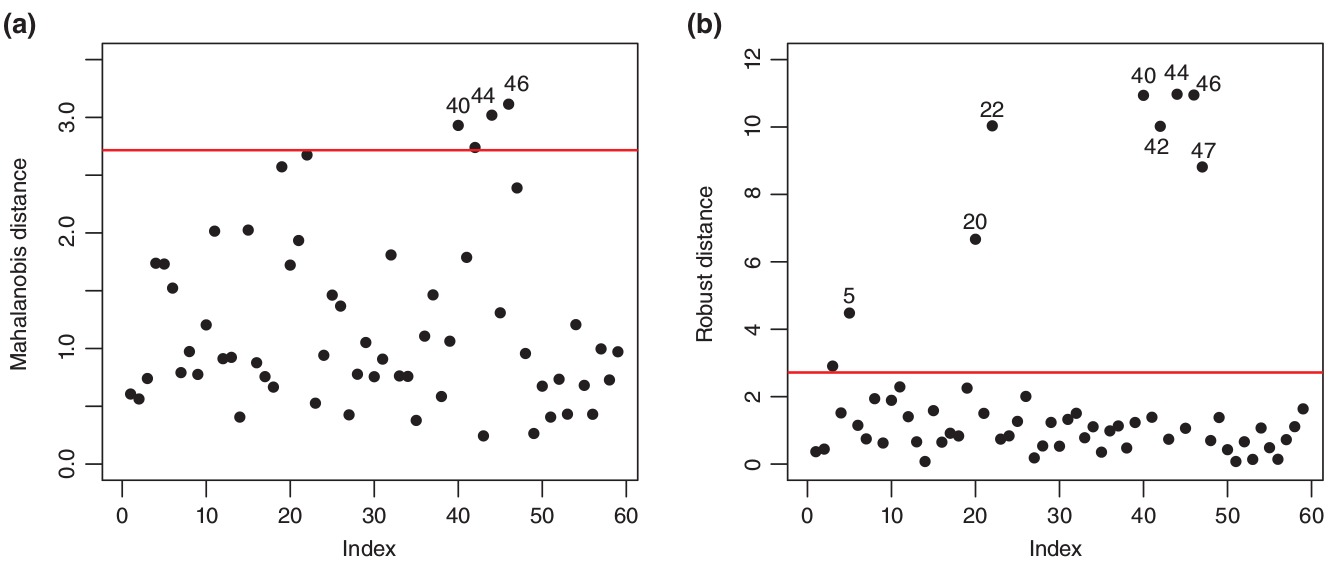
\includegraphics[width=11cm]{figures/mahalanobis_robust.png}
     \caption{Mahalanobis Distance for non-robust and robust estimates.}
     \label{fig:fig04}
\end{figure}

\begin{figure}[h!]
     \centering
     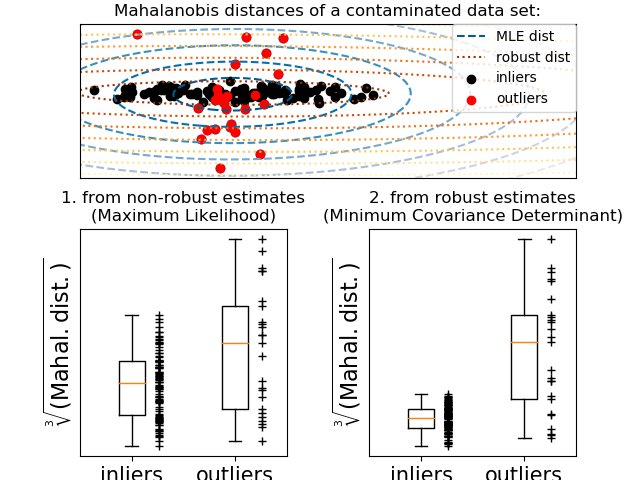
\includegraphics[width=8cm]{figures/mahalanobis_distances01.png}
     \caption{Mahalanobis Distance for non-robust and robust estimates.}
     \label{fig:fig05}
\end{figure}

The MCD estimator is one of the first affine equivariant and highly robust estimators of multivariate location and scatter.
		
Affine equivariant means that when the data are translated or subjected to a linear transformation, the resulting location and scatter will transform accordingly \cite{rousseeuw1984mcd,rousseeuw1999fastmcd}.

Its objective is to find $h$ observations (out of $n$) whose covariance matrix has the lowest determinant.

The lowest determinant means the lowest distance generalized variance and high distance between the largest eigenvalue and the remaining [ref?].

MCD depends on random sampling, therefore it is not deterministic.

MCD has been applied in numerous fields (medicine, finance, image analysis, and chemistry) and been used to develop many robust multivariate techniques (such as Robust Principal Component Analysis (RPCA), factor analysis, and multiple regression).

The classical MCD has rarely been applied because it is hard to compute, since it requires the evaluation of all $\binom{n}{h}$ subsets of size $h$. % binomial of n over p

Its main use has started since the construction of the computationally efficient Fast-MCD algorithm \cite{rousseeuw1999fastmcd}.

Fast-MCD is an iterative, approximate and resampling algorithm for the MCD.

It starts by random initial subset of size $p+1$ and performs concentration steps (C-steps) yielding consecutive h-subsets with decreasing covariance matrix determinant.

Only two C-steps are applied to each initial subset, and the 10 results with lowest determinant are kept.

C-steps are carried out until convergence and the best solution is kept.

Fast-MCD also is affine equivariant and not deterministic.
	
\textbf{Theorem 1: C-Step.} 

Consider a data set $\boldsymbol{X} \in \mathbb{R}^{n \times p}$ where $\boldsymbol{X} = \{\boldsymbol{x}_1,...,\boldsymbol{x}_n\}$ of $p$-variate observations. Let $\boldsymbol{h} \subset \{1,...,n\}$ with $|\boldsymbol{h}| = h$, where $\boldsymbol{h}$ is a subset of $h$ indexes from $n$ observations.

Let the mean $\bar{\boldsymbol{x}} \in \mathbb{R}^{1 \times p}$ be

\begin{equation}\label{eq:eq02}
	\bar{\boldsymbol{x}} = \displaystyle\frac{1}{h}\displaystyle\sum_{j\in \boldsymbol{h}} \boldsymbol{x}_j, 
\end{equation}

the covariance matrix $\boldsymbol{\hat{S}} \in \mathbb{R}^{p \times p}$ be

\begin{equation}\label{eq:eq03}
	\boldsymbol{\hat{S}} = \displaystyle\frac{1}{h}\displaystyle\sum_{j\in \boldsymbol{h}} (\boldsymbol{x}_j - \bar{\boldsymbol{x}})(\boldsymbol{x}_j - \bar{\boldsymbol{x}})^\prime,
\end{equation}

and the relative distance be 	

\begin{equation}\label{eq:eq04}
	\boldsymbol{d}(i) = \sqrt{(\boldsymbol{x}_i - \bar{\boldsymbol{x}}) \boldsymbol{\hat{S}}^{-1}(\boldsymbol{x}_i - \bar{\boldsymbol{x}})^\prime}, 
\end{equation}

for $i = 1,...,n$.

Let $\boldsymbol{h}_1, \bar{\boldsymbol{x}}_1$ and $\boldsymbol{\hat{S}}_1$ and be the selected observations, the location and scatter of the initial subset, and $\boldsymbol{d}_1(i)$ be the initial distances for $i = 1,...,n$. 

Now take $\boldsymbol{h}_2$ containing the indexes of lowest distances, such that $\{\boldsymbol{d}_1(i); i \in \boldsymbol{h}_2\} = \{(\boldsymbol{d}_1)_{1:n},...,(\boldsymbol{d}_1)_{h:n}\}$, where $(\boldsymbol{d}_1)_{1:n} \leq (\boldsymbol{d}_1)_{2:n} \leq ... \leq (\boldsymbol{d}_1)_{n:n}$ are the ordered distances, and compute $\boldsymbol{\bar{x}}_2$ and $\boldsymbol{\hat{S}}_2$ for $\boldsymbol{h}_2$.
	
Then, $det(\boldsymbol{\hat{S}}_2) \leq det(\boldsymbol{\hat{S}}_1)$ with equality if and only if $\boldsymbol{\bar{x}}_2 = \boldsymbol{\bar{x}}_1$ and $\boldsymbol{\bar{S}}_2 = \boldsymbol{\hat{S}}_1$

The proof is given by Rousseeuw and Driessen \cite{rousseeuw1999fastmcd}.
	
\textbf{The C-step can be algorithmically described as follows:}
\begin{algorithm}
	\label{alg:alg01}
	\scriptsize
	\SetAlgoLined
	\KwResult{$\boldsymbol{\bar{x}}_2$, $\boldsymbol{\hat{S}}_2$}
	Given the initial $h-$subset $\boldsymbol{h}_1$ of indexes or the pair $(\boldsymbol{\bar{x}}_1, \boldsymbol{\hat{S}}_1)$\;
	\While{$det(\boldsymbol{\hat{S}}_2) < det(\boldsymbol{\hat{S}}_1)$}{
		\If{$\boldsymbol{\bar{x}}_2$ and $\boldsymbol{\hat{S}}_2$ exist}{
			Put $\boldsymbol{\bar{x}}_1 = \boldsymbol{\bar{x}}_2$ and $\boldsymbol{\hat{S}}_1 = \boldsymbol{\hat{S}}_2$\;
		}
		Compute the distances $\boldsymbol{d}_1( i )$ for $i = 1,..., n$\;
		Sort $\boldsymbol{d}_1( i )$, which yields an index $\boldsymbol{d}_1(\pi(1)) \leq ... \leq \boldsymbol{d}_1(\pi(n))$\;
		Put $\boldsymbol{h}_2 = \{ \pi(1), \pi(2), ..., \pi(h)\}$\;
		Compute $\boldsymbol{\bar{x}}_2$ and $\boldsymbol{\hat{S}}_2$ for $\boldsymbol{h}_2$\;
		Compute $det(\boldsymbol{\hat{S}}_2)$ and $det(\boldsymbol{\hat{S}}_1)$\;			
	}
	\caption{C-Step}
\end{algorithm}

\textbf{Theorem 1} thus provides a partial idea for an algorithm: 

\textit{Take many initial choices of $\boldsymbol{h}_1$ and apply C-steps to each until convergence (don't have determinant decreasing), and keep the result with lowest determinant}.

\textbf{Initial subset can be algorithmically described as:}
\begin{algorithm}
	\label{alg:alg02}
	\scriptsize
	\SetAlgoLined
	\KwResult{$\boldsymbol{h}_1$}
	Given a data set $\boldsymbol{X} \in \mathbb{R}^{n \times p}$ with $p$-variate observations\;
	Draw a random $(p + 1)$-subset $\boldsymbol{L}$\;
	Compute $\boldsymbol{\bar{x}}_1$ and $\boldsymbol{\hat{S}}_1$ of $\boldsymbol{L}$ and $det(\boldsymbol{\hat{S}}_1)$\;
	\If{$det(\boldsymbol{\hat{S}}_1) \leq 0$}{
		Add another random observation into $\boldsymbol{L}$\;
		Compute $\boldsymbol{\bar{x}}_1$ and $\boldsymbol{\hat{S}}_1$ of $\boldsymbol{L}$ and $det(\boldsymbol{\hat{S}}_1)$\;
	}
	Compute $\boldsymbol{d}_1^2(i) = (\boldsymbol{x}_i - \boldsymbol{\bar{x}}_1)^\prime \boldsymbol{\hat{S}}_1^{-1}(\boldsymbol{X}_i - \boldsymbol{\bar{x}}_0)$ for $i = 1, ..., n$\;
	Sort them into $\boldsymbol{d}_1(\pi(1)) \leq ... \leq \boldsymbol{d}_0(\pi(n))$\;
	Put $\boldsymbol{h}_1 = \{\pi(1), ..., \pi(h)\}$\;
	\caption{Constructing the initial subset}
\end{algorithm}

\begin{algorithm}
	\label{alg:alg03}
	\scriptsize
	\SetAlgoLined
	\KwResult{$\boldsymbol{\bar{x}}_2$, $\boldsymbol{\hat{S}}_2$}
	Given $\boldsymbol{X} \in \mathbb{R}^{n \times p}$, $h < n$, $p \geq 2$ and $n \leq 600$\;
	\For{500 times}{
		Construct initial $h$-subset $\boldsymbol{h}_1$ (Algorithm \ref{alg:alg02})\;
		Carry out two C-steps (Algorithm \ref{alg:alg01}) resulting $\boldsymbol{\bar{x}}_2$ and $\boldsymbol{\hat{S}}_2$\;
	}		
	Put $\boldsymbol{h}_1$ as the 10 lowest $det(\boldsymbol{\hat{S}_2})$ computed above\;
	\While{$det(\boldsymbol{\hat{S}}_2) < det(\boldsymbol{\hat{S}}_1)$}{
		Carry out C-steps (Algorithm \ref{alg:alg01})\;
	}
	\caption{Fast-MCD when $n \leq 600$}
\end{algorithm}

\begin{algorithm}
	\label{alg:alg04}
	\scriptsize
	\SetAlgoLined
	\KwResult{$\boldsymbol{\bar{x}}_2$, $\boldsymbol{\hat{S}}_2$}
	Given $\boldsymbol{X} \in \mathbb{R}^{n \times p}$, $h < n$, $p \geq 2$ and $n > 600$\;
	Construct up to 5 disjoint random subsets of size $n_{sub} = 300$\;
	\For{each subset, repeat 100 times}{
		Construct initial $\boldsymbol{h}_1$ of size $h_{sub} = [n_{sub}(h/n)]$\;
		Carry out two C-steps of $n_{sub}$ and $h_{sub}$\;
		Keep the 10 best $(\boldsymbol{\bar{x}}_{sub}, \boldsymbol{\hat{S}}_{sub})$\;
	}		
	Pool the subsets, yielding the merged set of $n_{merged} = 1500$\;
	\For{50 best $(\boldsymbol{\bar{x}}_{sub}, \boldsymbol{\hat{S}}_{sub})$}{
		Carry out two C-steps of $n_{merged}$ and $h_{merged} = [n_{merged}(h/n)]$\;
		Keep the 10 best $(\boldsymbol{\bar{x}}_{merged}, \boldsymbol{\hat{S}}_{merged})$\;
	}
	\For{the full data set and $m_{full}$ best results}{
		Take several C-steps, using $n$ and $h$\;
		Keep the best final result $(\boldsymbol{\bar{x}}_{full}, \boldsymbol{\hat{S}}_{full})$\;
	}
	\caption{Fast-MCD when $n > 600$}
\end{algorithm}

Our proposal is ...

%%%%%%%%%%%%%%%%%%%%%%%%%%%%%%%%%%%%%%%%%%%%%%%%%%%%%%%%%%%%%%%%%%%%%%%%%%%%%%%%%%%%%%%%%%%%%%%%%%%%%%%%%%%%%%%%%%%%%%%%%%%%%%%%%%%%%%%%%%%%%%%%%%%%%%%%%%%%%%%%%%%%%%%%%%%%%%%%%%%%%%%%%%%%%%%%%%%%%%%%%%%%%%%%%%%%%%%%%%%%
\section{Data Model}
\label{sec:datamodel}

In this paper, scalars are denoted by italic letters (\emph{a, b, A, B, $α$, $β$}), vectors by lowercase bold letters (\textbf{a, b}), matrices by uppercase bold letters (\textbf{A, B}), and $a_i,_j$ denotes the (\emph{i, j}) elements of the matrix \textbf{A}. The superscripts \textsuperscript{T} and \textsuperscript{-1} are used for matrix transposition and matrix inversion, respectively. We define the operator $\rm diag(\cdot)$ that returns the vector of the main diagonal of a given matrix, the operator $\rightarrow$, which denotes the deletion of a given element from a set and the operator $\#$, that returns the rank of a matrix, and the operator $\sim$ that sorts the elements of a vector in ascending order.

This section also presents a description of the data model and data aggregation of the CTU-13 data set, in Subsection \ref{sec:CTU-13} discusses the use of the CTU-13 data set for evaluation of the proposed approach.

\subsection{The CTU-13 data set}
\label{sec:CTU-13}


\cite{garcia2014empirical} proposed CTU-13 data set and argues that for evaluations of anomaly detection, none of the botnet families used in the training and crossvalidation data set should be used in the testing data set, considering that this ensures that the methods can generalize and detect new behaviors. However, hour proposal is semi-supervised and does not rely on training data with anomalies. Adopting the training and testing approach of \cite{garcia2014empirical}, some botnets malware wouldnt be evaluated, since in Garcia's proposal some botnets are present only for training. Therefore, we evaluate each scenario individually.


A. Description of CTU-13 data set
The CTU-13 is a data set of botnet traffic that was captured
in the Czech Technical University [24]. It contains 13 scenarios
with various botnet types. We consider scenarios 1, 2, 6, 8, and
9 of the data set.
• Scenario 1 corresponds to an IRC-based botnet that sent
spam for almost 6.5 hours.
• Scenario 2 (2.5-hours) is from the same botnet.
• Scenario 6 is from a botnet that scanned SMTP (Simple
Mail Transfer Protocol) servers for 2 hours and connected
to several RDP (Remote Desktop Protocol) services. Dif-
ferent with Scenarios 1 and 2, this botnet neither sent
spam nor did it attack. It’s C\&C server used a proprietary
protocol.
• Scenario 8 is from a botnet that contacted a lot of Chinese
C\&C hosts and received large amounts of encrypted data.
The botnet also cracked the passwords of machines during
the 19-hour attack.
• Scenario 9 corresponds to a case where 10 local hosts
were infected by a spamming botnet. More than 600 spams
were sent over 5 hours.
For all the scenarios, the authors of the CTU-13 data set
convert the captured pcap files to NetFlows and release the
processed flows. The data set contains ground-truth labels for
flows as follows: flows from or to the infected machines
are labeled as “botnet”; flows from or to noninfected ma-
chines are labeled as “normal”; all other flows are labeled as
“background.”

Evaluating network anomaly detection solutions remains a challenge due to the lack of up-to-date real-world data sets for training and testing \cite{osanaiye2016distributed}. 

We propose to use CTU-13 \cite{garcia2014empirical} to evaluate our proposal, considering that the CTU-13 is a data set that aims to have a large capture of real botnet attacks and C\&C traffic mixed with normal and background traffic.

The CTU-13 data set consists in thirteen captures (called scenarios) of different botnet samples. 

On each scenario it was executed a specific malware, which used several protocols and performed different actions.		

The botnet traffic is divided into attacks and Command and Control (C\&C) traffic.

\textbf{Attacks:} Click Fraud, Port Scan, FastFlux, Compiled and Controled by Authors, SPAM and DDOS.

\textbf{C\&C:} IRC, P2P and HTTP.

The data set contains the following features:  Start Time, End Time, Duration, Source IP address, Source Port, Direction, Destination IP address, Destination Port, State, SToS, Total Packets and Total Bytes.

Start Time, Duration, Protocol, Source Address, Source Port, Direction, Destination Address, Destination Port, State, Type of service from source to destination, Type of service from destination to source, Total of Packets, Total of bytes, Total bytes from source to destination, Label as normal or anomalous

Our labeling strategy assigns three different labels: back-ground, botnet and normal. The priority to assign the labels is the following: 1. Assign the Background label to the whole traffic. 2. Assign the Normal label to the traffic that matches certain filters. 3. Assign the Botnet label to all the traffic that comes from or to any of the known infected IP addresses.

\begin{table}[h!]
	\tiny
	\caption{CTU-13 data set Description}
	\label{tab:tab01}
	\begin{tabular}{| l | l | l | l | l | l | l | l | l | l | l | }
		\hline \rowcolor{Gray} \begin{tabular}[x]{@{}l@{}}Scenario\end{tabular}	& \begin{tabular}[x]{@{}l@{}}Malware\end{tabular}	 & \begin{tabular}[x]{@{}l@{}}Type\end{tabular}	& \begin{tabular}[x]{@{}l@{}}Total Flows\end{tabular} & \begin{tabular}[x]{@{}l@{}}Malicious\end{tabular} & \begin{tabular}[x]{@{}l@{}}C\&C\end{tabular} & \begin{tabular}[x]{@{}l@{}}Botnet\end{tabular}\\ \hline
			10 & neris & IRC, Spam, CF & 2,824,636 & 40,961 (1.45\%) & 341 (0.01\%) & 40,620 (1.44\%) \\ \hline
			11 & neris & IRC, Spam, CF & 1,808,122 & 20,941 (1.16\%) & 673 (0.04\%) & 20,268 (1.12\%) \\ \hline
			12 & rbot & IRC, PS, US & 4,710,638 & 26,822 (0.57\%) & 63 (0.00\%) & 26,759 (0.57\%) \\ \hline
			15 & rbot & IRC, DDoS, US & 1,121,076 & 2,580 (0.23\%) & 52 (0.00\%) & 2,528 (0.23\%) \\ \hline
			15-2 & virut & Spam, PS,HTTP & 129,832 & 901 (0.69\%) & 24 (0.02\%) & 877 (0.68\%) \\ \hline
			16 & menti & PS & 558,919 & 4,630 (0.83\%) & 199 (0.04\%) & 4,431 (0.79\%) \\ \hline
			16-2 & sogou & HTTP & 114,077 & 63 (0.06\%) & 26 (0.02\%) & 37 (0.03\%) \\ \hline
			16-3 & murlo & PS & 2,954,230 & 6,127 (0.21\%) & 1,074 (0.04\%) & 5,053 (0.17\%) \\ \hline
			17 & neris & IRC, Spam, CF,PS & 2,087,508 & 184,987 (8.86\%) & 2,973 (0.14\%) & 182,014 (8.72\%) \\ \hline
			18 & rbot & IRC, DDoS, US & 1,309,791 & 106,352 (8.12\%) & 33 (0.00\%) & 106,319 (8.12\%) \\ \hline
			18-2 & rbot & IRC, DDoS, US & 107,251 & 8,164 (7.61\%) & 2 (0.00\%) & 8,162 (7.61\%) \\ \hline
			19 & nsys.ay & P2P & 325,471 & 2,168 (0.67\%) & 25 (0.01\%) & 2,143 (0.66\%) \\ \hline
			15-3 & virut & Spam, PS, HTTP & 1,925,149 & 40,003 (2.08\%) & 536 (0.03\%) & 39,467 (2.05\%) \\ \hline
	\end{tabular}
\end{table}

Table \ref{tab:tab01} presents the malwares used for botnet attacks, the attack and C\&C types, the total number of flows, the number of malicious flows, which includes the C\&C and botnet flows. Table \ref{tab:tab01} also shows the ratio of C\&C and botnet flows.

Table \ref{tab:tab01} shows that CTU-13 is very imbalanced data set, when comparing the amount of malicious to normal traffic.

Malicious observations are beteeen $0.06\%$ up to $8.86\%$ of all flows.

The scenarios have between $107,251$ and $4,710,638$ flows.

The CTU-13 data set is also very skewed. Figure \ref{fig:fig06} exemplifies the skewed distribution of normal and anomalous flows, showing the flow duration of scenario 12.

\begin{figure}[h!]
     \centering
     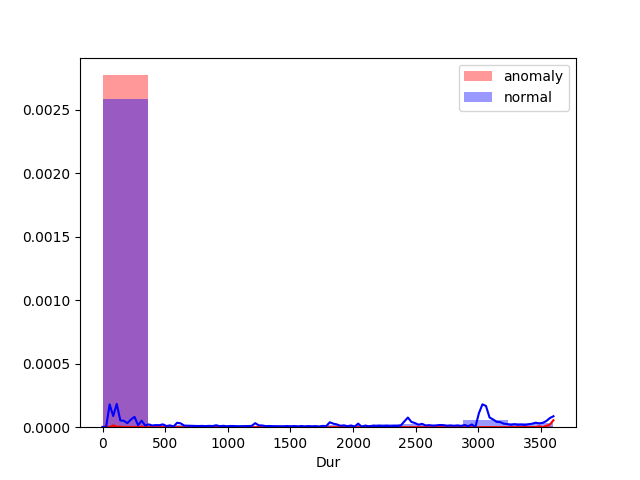
\includegraphics[width=8cm]{figures/raw_distplot_capture20110812_Dur.png}
     \caption{Distribution of flow duration for scenario 12.}
     \label{fig:fig06}
\end{figure}
	
Methods for imbalance learning has attracted growing attention from both academia and industry, due to the restrictions imposed by imbalanced data to machine learning algorithms.

Lakhina et al. \cite{lakhina2005mining} argue that the distributions of packet features (IP addresses and ports) observed in flow traces reveals both the presence and the structure of a wide range of anomalies.

To deal with the data imbalance of CTU-13 data set, we adopt a sampling method based on data aggragation for feature generation, in order to obtain less imbalanced and more discrimnative data. Based on related works \cite{lakhina2005mining,gu2008botminer,callegari2011novel,chandrashekar2014survey,garcia2014empirical,acarali2016survey} and experience \cite{vieira2017model, galibus2017offline}, we selected some features for improving the anomaly detection.
The features are generated by a data aggregation into a selected window size. We evalute our proposal for windows with 0.15 and 0.25 seconds, for each scenario of the CTU-13 data set.
	
Following (2 slides) are the selected features:
\textbf{normal-flow-count:} count of normal (known) flow.
\textbf{background-flow-count :} count of background (unknown) flows.
\textbf{avg-duration:} average duration time of flows.
\textbf{n-conn:} count of flows.
\textbf{n-icmp:} count of ICMP packets.
\textbf{n-tcp:} count of TCP packets.
\textbf{n-udp:} count of UDP packets.
\textbf{n-dports<1024:} count of destinations ports lower than 1024.
\textbf{n-sports<1024:} count of source ports lower than 1024.
\textbf{n-sports>1024:} count of source ports higher than 1024.

Following are the remaining selected features:
\textbf{n-s-a-p-address:} count of class A source address.
\textbf{n-d-a-p-address:} count of class A destination address.
\textbf{n-s-b-p-address:} count of class B source address.
\textbf{n-d-b-p-address:} count of class B destination address.
\textbf{n-s-c-p-address:} count of class C source address.
\textbf{n-d-c-p-address:} count of class C destination address.
\textbf{n-s-na-p-address:} count of class D* source address.
\textbf{n-d-na-p-address:} count of class D* destination address.

Figures \ref{fig:fig07} and \ref{fig:fig08} show the distribution of average flow duration, for scenario 12, aggregated by windows of 0.15 and 2 seconds.

In comparison to Figure \ref{fig:fig06}, that shows the distribution of flow duration for the same scenario, we can see that the feature based on the average is more discriminative.

\begin{figure}[h!]
     \centering
     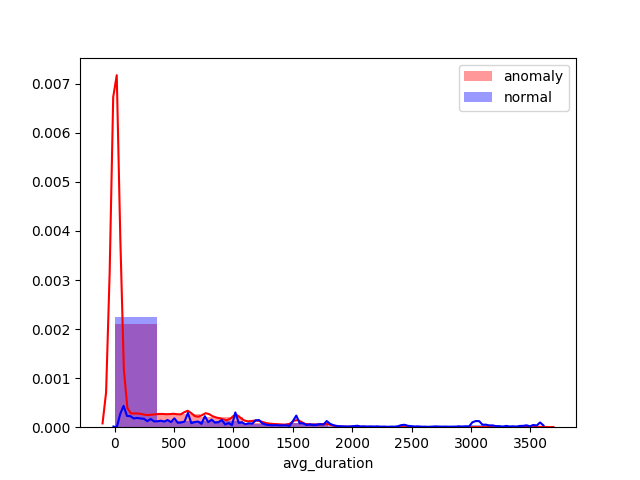
\includegraphics[width=8cm]{figures/agg_distplot_0_15s_12_avg_duration.png}
     \caption{Distribution of average flow duration for scenario 12, aggregated by windows of 0.15 seconds.}
     \label{fig:fig07}
\end{figure}

\begin{figure}[h!]
     \centering
     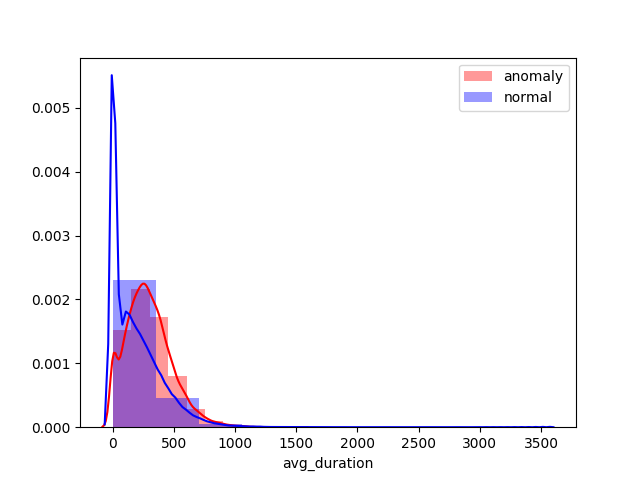
\includegraphics[width=8cm]{figures/agg_distplot_2s_12_avg_duration.png}
     \caption{Distribution of average flow duration for scenario 12, aggregated by windows of 2 seconds.}
     \label{fig:fig08}
\end{figure}


%%%%%%%%%%%%%%%%%%%%%%%%%%%%%%%%%%%%%%%%%%%%%%%%%%%%%%%%%%%%%%%%%%%%%%%%%%%%%%%%%%%%%%%%%%%%%%%%%%%%%%%%%%%%%%%%%%%%%%%%%%%%%%%%%%%%%%%%%%%%%%%%%%%%%%%%%%%%%%%%%%%%%%%%%%%%%%%%%%%%%%%%%%%%%%%%%%%%%%%%%%%%%%%%%%%%%%%%%%%%
\section{Robust PCA and Higher Moments Distances for Botnet Detection}
\label{sec:m_rpca}

This section describes the proposed technique to detect synflood, fraggle and port scan, according to Figure \ref{fig:fig80}, which represents the overview of the proposed framework for detection and identification of network attacks. In Subsection \ref{sec:prop_LargestEigenvaluebyTimeFrames} we present the steps for extraction of the largest eigenvelue for each $q$-th time frame. Next, in Subsection \ref{sec:prop_MOSSchemes}, we show how to apply the eiganvalues on the MOS scheme in order to detect the attack. In Subsection \ref{sec:prop_EigenvalueAnalysis}, we present the eigenvalue analysis to identify the time frames detected as under attack, and the Subsection \ref{sec:prop_EigenSimilarityAnalysis} describes the similarity analysis evaluated for detailed attack identification.

\begin{figure}[h!]
	\centering
     % 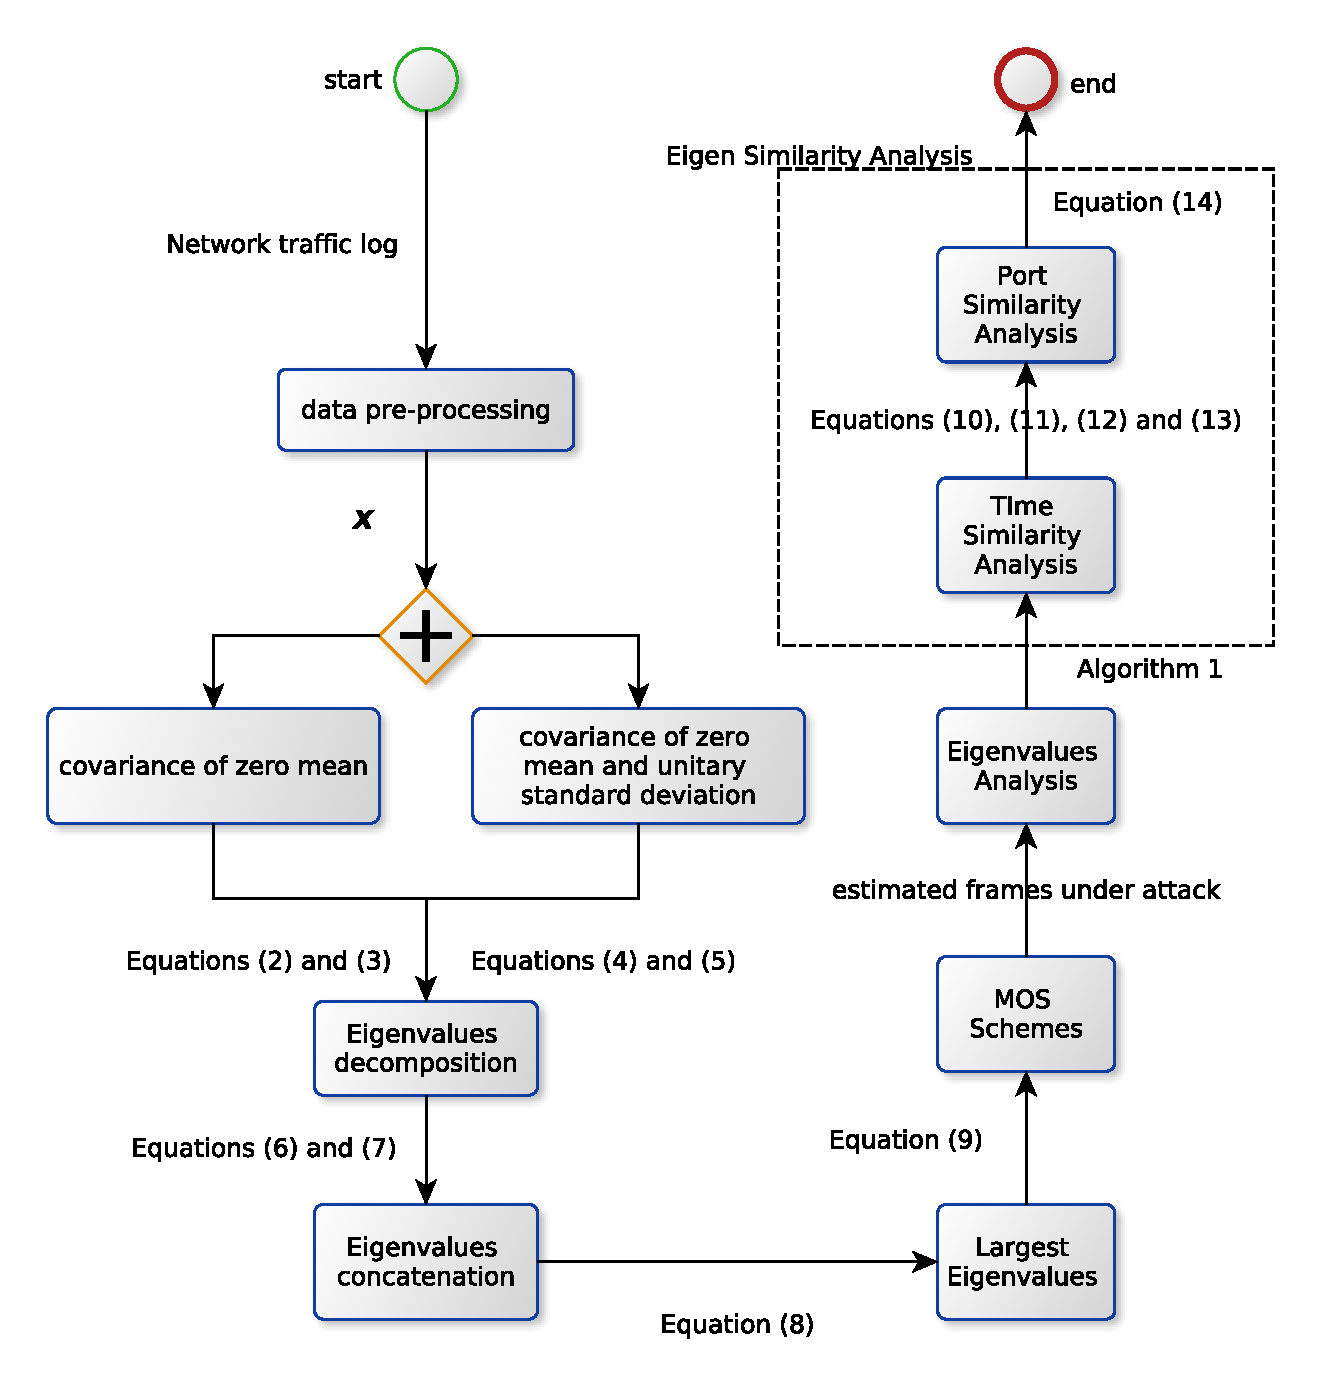
\includegraphics[height=11cm, width=9cm]{results/figures/mos_eigen_similarity.eps}
     \caption{Overview of The Framework for Detection and Identification of Network Attacks.}
     \label{fig:fig80}
\end{figure}

\subsection{Largest Eigenvalue by Time Frames}
\label{sec:prop_LargestEigenvaluebyTimeFrames}

We propose to extend Fast-MCD for computing robust moments (skewness and kurtosis), in order to improve the anomaly detection in a skewed and imbalanced data set of network traffic with normal and botnet traffic.
	    
Moments are a set of statistical parameters to measure a distribution. The arithmetic mean is the first general moment, the second is the variance, while skewness (asymmetry) is the third moment and kurtosis (excess) is the fourth moment.

The general formula of the $r$-th moment can be expressed as:
\begin{equation}\label{eq:eq05}
	m_r = \displaystyle\frac{1}{n}\displaystyle\sum_{i = 1}^{n}( x_i - \bar{x})^r. 
\end{equation}

Therefore, the Skewness is calculated as
\begin{equation}\label{eq:eq06}
	\boldsymbol{\bar{s}} = \frac{m_3}{m_2^{\frac{3}{2}}},
\end{equation}

and Kurtosis as
\begin{equation}\label{eq:eq07}
	\boldsymbol{\bar{k}} = \frac{m_4}{m_2^2} 
\end{equation}

For extending Fast-MCD, We initially modify the C-step Algorithm \ref{alg:alg01} to calculate Skewness and Kurtosis after to minimize $det(\boldsymbol{\hat{S}})$, accordingly to Algorithm \ref{alg:alg05}.

\begin{algorithm}
	\label{alg:alg05}
	\scriptsize
	\SetAlgoLined
	\KwResult{$\boldsymbol{\bar{x}}_2$, $\boldsymbol{\hat{S}}_2$, $\boldsymbol{\bar{s}}_2$ and $\boldsymbol{\bar{k}}_2$}
	Given the initial $h-$subset $\boldsymbol{h}_1$ of indexes or the pair $(\boldsymbol{\bar{x}}_1, \boldsymbol{\hat{S}}_1)$\;
	\While{$det(\boldsymbol{\hat{S}}_2) < det(\boldsymbol{\hat{S}}_1)$}{
		\If{$\boldsymbol{\bar{x}}_2$ and $\boldsymbol{\hat{S}}_2$ exist}{
			Put $\boldsymbol{\bar{x}}_1 = \boldsymbol{\bar{x}}_2$ and $\boldsymbol{\hat{S}}_1 = \boldsymbol{\hat{S}}_2$\;
		}
		Compute the distances $\boldsymbol{d}_1( i )$ for $i = 1,..., n$\;
		Sort $\boldsymbol{d}_1( i )$, which yields an index $\boldsymbol{d}_1(\pi(1)) \leq ... \leq \boldsymbol{d}_1(\pi(n))$\;
		Put $\boldsymbol{h}_2 = \{ \pi(1), \pi(2), ..., \pi(h)\}$\;
		Compute $\boldsymbol{\bar{x}}_2$ and $\boldsymbol{\hat{S}}_2$ for $\boldsymbol{h}_2$\;
		Compute $det(\boldsymbol{\hat{S}}_2)$ and $det(\boldsymbol{\hat{S}}_1)$\;			
	}
	Compute $\boldsymbol{\bar{s}}_2$ and $\boldsymbol{\bar{k}}_2$ for last $\boldsymbol{h}_2$\;
	\caption{C-Step with higher moments}
\end{algorithm}

The Algorithm \ref{alg:alg06} describes the Fast-MCD with higher moments when $n \leq 600$, through the modification of the original Fast-MCD for computing Skewness and Kurtosis from the robust estimate.
    
\begin{algorithm}
	\label{alg:alg06}
	\scriptsize
	\SetAlgoLined
	\KwResult{$\boldsymbol{\bar{x}}_2$, $\boldsymbol{\hat{S}}_2$, $\boldsymbol{\bar{s}}_2$ and $\boldsymbol{\bar{k}}_2$}
	Given $\boldsymbol{X} \in \mathbb{R}^{n \times p}$, $h < n$, $p \geq 2$ and $n \leq 600$\;
	\For{500 times}{
		Construct initial $h$-subset $\boldsymbol{h}_1$ (Algorithm \ref{alg:alg02})\;
		Carry out two C-steps with higher moments (Algorithm \ref{alg:alg05}) resulting $\boldsymbol{\bar{x}}_2$, $\boldsymbol{\hat{S}}_2$, $\boldsymbol{\bar{s}}_2$ and $\boldsymbol{\bar{k}}_2$\;
	}		
	Put $\boldsymbol{h}_1$ as the 10 lowest $det(\boldsymbol{\hat{S}_2})$ computed above\;
	\While{$det(\boldsymbol{\hat{S}}_2) < det(\boldsymbol{\hat{S}}_1)$}{
		Carry out C-steps with higher moments (Algorithm \ref{alg:alg05})\;
	}
	\caption{Fast-MCD with higher moments when $n \leq 600$}
\end{algorithm}

The Algorithm \ref{alg:alg07} presents the Fast-MCD with higher moments when $n > 600$, which modifies the original Fast-MCD for computing of Skewness and Kurtosis from the robust estimate data, through the adoption of the C-Step with higher moments. The Algorithm \ref{alg:alg07} is described below.

\begin{algorithm}
	\label{alg:alg07}
	\scriptsize
	\SetAlgoLined
	\KwResult{$\boldsymbol{\bar{x}}_2$, $\boldsymbol{\hat{S}}_2$, $\boldsymbol{\bar{s}}_2$ and $\boldsymbol{\bar{k}}_2$}
	Given $\boldsymbol{X} \in \mathbb{R}^{n \times p}$, $h < n$, $p \geq 2$ and $n > 600$\;
	Construct up to 5 disjoint random subsets of size $n_{sub} = 300$\;
	\For{each subset, repeat 100 times}{
		Construct initial $\boldsymbol{h}_1$ of size $h_{sub} = [n_{sub}(h/n)]$\;
		Carry out two C-steps with higher moments of $n_{sub}$ and $h_{sub}$\;
		Keep the 10 best $(\boldsymbol{\bar{x}}_{sub}, \boldsymbol{\hat{S}}_{sub}, \boldsymbol{\bar{s}}_{sub}, \boldsymbol{\bar{k}}_{sub})$\;
	}		
	Pool the subsets, yielding the merged set of $n_{merged} = 1500$\;
	\For{50 best $(\boldsymbol{\bar{x}}_{sub}, \boldsymbol{\hat{S}}_{sub})$}{
		Carry out two C-steps with higher moments of $n_{merged}$ and $h_{merged} = [n_{merged}(h/n)]$\;
		Keep the 10 best $(\boldsymbol{\bar{x}}_{merged}, \boldsymbol{\hat{S}}_{merged}, \boldsymbol{\bar{s}}_{merged}, \boldsymbol{\bar{k}}_{merged})$\;
	}
	\For{the full data set and $m_{full}$ best results}{
		Take several C-steps, using $n$ and $h$\;
		Keep the best final result $(\boldsymbol{\bar{x}}_{full}, \boldsymbol{\hat{S}}_{full}, \boldsymbol{\bar{s}}_{full}, \boldsymbol{\bar{k}}_{full})$\;
	}
	\caption{Fast-MCD with higher moments when $n > 600$}
\end{algorithm}

We also propose to use Mahalanobis Distance for detecting anomalies through an approach based on robust Skewness and Kurtosis, instead of the location and scatter that are used by classical approaches.

We propose to modify the Equation \ref{eq:eq01} to implement a Skewness-based Mahalanobis Distance, as follows:

\begin{equation}\label{eq:eq08}
	\boldsymbol{d}(\boldsymbol{s}_{\boldsymbol{x}}, \bar{\boldsymbol{s}}, \boldsymbol{\hat{S}}) = \sqrt{(\boldsymbol{s}_{\boldsymbol{x}} - \bar{\boldsymbol{s}}) \boldsymbol{\hat{S}}^{-1}(\boldsymbol{s}_{\boldsymbol{x}} - \bar{\boldsymbol{s}})^\prime}, 
\end{equation}

where $\boldsymbol{s}_{\boldsymbol{x}} = \boldsymbol{x} - \boldsymbol{\bar{s}}(\boldsymbol{x})$ and $\boldsymbol{\bar{s}}(\boldsymbol{x})$ is the Skewness of $\boldsymbol{x}$.

We also propose to modify the Equation \ref{eq:eq04} to implement a Kurtosis-based Mahalanobis Distance, as follows:

\begin{equation}\label{eq:eq09}
	\boldsymbol{d}(\boldsymbol{k}_{\boldsymbol{x}}, \bar{\boldsymbol{k}}, \boldsymbol{\hat{S}}) = \sqrt{(\boldsymbol{k}_{\boldsymbol{x}} - \bar{\boldsymbol{k}}) \boldsymbol{\hat{S}}^{-1}(\boldsymbol{k}_{\boldsymbol{x}} - \bar{\boldsymbol{k}})^\prime}, 
\end{equation}

where $\boldsymbol{k}_{\boldsymbol{x}} = \boldsymbol{x} - \boldsymbol{\bar{k}}(\boldsymbol{x})$ and $\boldsymbol{\bar{k}}(\boldsymbol{x})$ is the Kurtosis of $\boldsymbol{x}$.

Fast-MCD is commonly used as \textbf{supervised} or \textbf{unsupervised} algorithm for anomaly detection.
		
\textbf{Supervised} approach:

Compute Fast-MCD for training data with known normal and anomalous data.
Select the best threshold $t$ for detecting known anomalies according to largest distances $\boldsymbol{d}(i)$.
Save the best $t, \boldsymbol{\bar{x}}$ and $\boldsymbol{\hat{S}}$.
Compute $d(\boldsymbol{x},\bar{\boldsymbol{x}}, \boldsymbol{\hat{S}})$ for new observations.
Classify observations with $\boldsymbol{d}(i)$ higher than $t$ as anomalous.

\textbf{Unsupervised} approach:

Given a known contamination $c$, which is the percentage of anomalies in a data set.
Compute Fast-MCD and $d(\boldsymbol{x},\bar{\boldsymbol{x}}, \boldsymbol{\hat{S}})$ for new observations.
Classify the $c$ observations with largest distances as anomalous.

Finally, We propose the following \textbf{Semi Supervised} approach for Fast-MCD based anomaly detection:

Compute Fast-MCD for training data containing only known normal observations.
Save the fitted $\boldsymbol{\bar{x}}_{normal}$ and $\boldsymbol{\hat{S}}_{normal}$.
Carry out cross validation on known contaminated data in order to identify the contamination $c$ that best classify anomalies and normal data.
Compute $d(\boldsymbol{x},\bar{\boldsymbol{x}}_{normal}, \boldsymbol{\hat{S}}_{normal})$ for new observations.
The $c$ observations with largest $\boldsymbol{d}(i)$ are classified as anomalous.


\subsection{MOS Schemes}
\label{sec:prop_MOSSchemes}

\subsection{Eigen Similarity Analysis}
\label{sec:prop_EigenSimilarityAnalysis}

\subsubsection{Time Similarity Analysis}
\label{sec:prop_TimeSimilarityAnalysis}

\subsubsection{Port Similarity Analysis}
\label{sec:prop_PortSimilarityAnalysis}

%%%%%%%%%%%%%%%%%%%%%%%%%%%%%%%%%%%%%%%%%%%%%%%%%%%%%%%%%%%%%%%%%%%%%%%%%%%%%%%%%%%%%%%%%%%%%%%%%%%%%%%%%%%%%%%%%%%%%%%%%%%%%%%%%%%%%%%%%%%%%%%%%%%%%%%%%%%%%%%%%%%%%%%%%%%%%%%%%%%%%%%%%%%%%%%%%%%%%%%%%%%%%%%%%%%%%%%%%%%%
\section{Experiments and Results}
\label{sec:experimentalresults}

This section presents the performed experiments and the acquired results. First, in Section \ref{sec:AnalyzedScenario}, the experimental scenario adopted in the experiments is summarized. Then, Section \ref{sec:largesteigenvaluesanalysis} shows the results of the largest eigenvalue analysis by time frames for the experimental scenario. In Section \ref{sec:MOSSchemesEvaluation} are described the results of the evaluated MOS schemes for attack detection in the simulated data set. Section \ref{sec:EigenvalueAnalysis} presents the results of the eigenvalue analysis for identification of time frames under attack, Section \ref{sec:EigenSimilarityAnalysis} shows the results of similarity analysis for detailed flood and port scan identification for the experimental scenario. Section \ref{sec:DarpaEvaluation} presents the results of the largest eigenvalue analysis, model order selection and the eigenvalue analysis for flood and probe attack detection in the DARPA 1998 data set.

\subsection{Experimental Scenario}
\label{sec:AnalyzedScenario}

\textbf{Experiment Plan:}

	Given a contaminated data set, split it into normal (60\%), cross validation (20\% normal + 50\% anomalous) and test (20\% normal + 50\% anomalous).
	Select the range of contamination that shall be evaluated and perform cross validation for each contamination. 
	For each contamination $c$:
	
		Estimate $\boldsymbol{\bar{x}}_{normal}$ and $\boldsymbol{\hat{S}}_{normal}$ from normal data.
		Predict anomalies for cross validation data using the $c$, $\boldsymbol{\bar{x}}_{normal}$ and $\boldsymbol{\hat{S}}_{normal}$.
		Select the best F-measure by cross validation and get the best $c$.
	
	Test the F-measure of anomaly detection for new observations through $d(\boldsymbol{x},\bar{\boldsymbol{x}}_0, \boldsymbol{\hat{S}}_0)$ and $c$.


\textbf{Experiment Plan:}

Evaluation Measure:

In anomalous detection problems, where anomalies are rare events, if we classify all observations as normal and apply an accuracy evaluation, we would have high accuracy but poor true-positive detection.

Due to the importance given by F-measure to true-positive detection \cite{powers2011evaluation,moustafa2019holistic}, the F-measure is the preferable measure for imbalanced data sets.

\textbf{Experiment Plan:}

	The F-measure is the harmonic mean of precision and recall and is defined by 
	\begin{equation}\label{eq:eq10}
		F-measure = 2 * \frac{PR * RC}{PR + RC},				
	\end{equation}
	where $PR$ is the precision, defined by 
	\begin{equation}\label{eq:eq11}
		PR = \frac{True Positive}{True Positive + False Positive}
	\end{equation}
	and $RC$ is the recall, defined by 
	\begin{equation}\label{eq:eq12}
		RC = \frac{True Positive}{True Positive + False Negative}.
	\end{equation}


\textbf{Data splitting for training, cross validation and testing}

	Gargia et al. \cite{garcia2014empirical} propose a division of CTU-13's scearios into train and test, for evaluation of network attack detection algorithms. 
	However, we decide to evaluate our proposed approach for each scenario individually, considering that in the division proposed by Gargia et al. some bots are present only for training and not for testing. 
	Although our proposal does not rely on anomalous data for training, we desire to evaluate our proposal to detect all types of bots captured by CTU-13 data set.




Why GMM?
As clustering-based method, we selected K-means, which is the clustering algorithm most adopted for general purposes and for network anomaly detection \cite{gaddam2007kmeans,moustafa2019holistic}.
It is observed that network traffic do not belong to a Gaussian distribution \cite{benson2010network,moustafa2019holistic}, algorithms based on non-Gaussian distributions, such as GMM, has been adopted for network anomaly detection \cite{moustafa2019holistic}.


\subsection{Results}
\label{sec:results}

\begin{table}[h!]
  \centering
  \scriptsize
  \caption{Results grouped by algorithm and scenario}
  \label{tab:tab02}
  \begin{tabular}{ c|c c|c c|c c|c c|c c }
	\toprule
	\multirow{2}{*}{\textbf{Scenario}}   &\multicolumn{2}{c}{\textbf{S-MCD}} &\multicolumn{2}{c}{\textbf{K-MCD}} &\multicolumn{2}{c}{\textbf{MCD}} &\multicolumn{2}{c}{\textbf{GMM}} &\multicolumn{2}{c}{\textbf{K-Means}}\\ 
			\hhline{~----------}
			&\textbf{0.15} &\textbf{0.25} &\textbf{0.15} &\textbf{0.25} &\textbf{0.15} &\textbf{0.25} &\textbf{0.15} &\textbf{0.25} &\textbf{0.15} &\textbf{0.25}\\
	\midrule
		10 &\color{red} 0.71 & 0.03 & 0.66 & 0.02 & 0.34 & 0.52 & 0.34 & 0.46 & 0.20 & 0.25 \\ \hline
		11 & 0.03 & 0.54 & 0.00 & 0.54 & 0.71 &\color{red} 0.73 & 0.35 & 0.48 & 0.13 & 0.15 \\ \hline
		12 & 0.19 & 0.02 & 0.20 & 0.05 & 0.06 &\color{red} 0.31 & 0.01 & 0.01 & 0.09 & 0.11 \\ \hline
		15 & 0.00 & 0.00 & 0.00 & 0.00 & 0.24 &\color{red} 0.32 & 0.14 & 0.22 & 0.09 & 0.11 \\ \hline
		15-2 & 0.04 & 0.85 & 0.67 &\color{red} 0.86 & 0.36 & 0.28 & 0.32 & 0.14 & 0.18 & 0.26 \\ \hline
		15-3 & 0.00 & 0.01 & 0.00 & 0.01 &\color{red} 0.55 & 0.48 & 0.00 & 0.01 & 0.22 & 0.29 \\ \hline
		16 & 0.45 & 0.36 & 0.42 & 0.33 & 0.27 & 0.41 &\color{red} 0.51 & 0.49 & 0.07 & 0.16 \\ \hline
		16-2 & 0.00 & 0.16 & 0.00 &\color{red} 0.20 & 0.04 & 0.04 & 0.02 & 0.08 & 0.04 & 0.03 \\ \hline
		16-3 & 0.00 & 0.05 & 0.00 & 0.07 &\color{red} 0.15 & 0.10 & 0.01 & 0.01 & 0.03 & 0.04 \\ \hline
		17 & 0.03 & 0.03 & 0.07 & 0.03 &\color{red} 0.59 & 0.53 & 0.16 & 0.47 & 0.35 & 0.39 \\ \hline
		18 & 0.63 & 0.10 & 0.63 & 0.08 & 0.70 &\color{red} 0.72 & 0.21 & 0.17 & 0.13 & 0.20 \\ \hline
		18-2 & 0.83 & 0.69 & 0.85 & 0.43 & 0.84 &\color{red} 0.91 & 0.50 & 0.55 & 0.62 & 0.70 \\ \hline
		19 &\color{red} 0.71 & 0.00 & 0.68 & 0.00 & 0.11 & 0.42 & 0.17 & 0.20 & 0.20 & 0.17 \\ \hline
		\rowcolor{Gray} \textbf{avg} & \textbf{0.28} & \textbf{0.22} & \textbf{0.32} & \textbf{0.20} & \textbf{0.38} &\color{red} \textbf{0.44} & \textbf{0.21} & \textbf{0.25} & \textbf{0.18} & \textbf{0.22} \\ 
    \bottomrule
  \end{tabular}
\end{table}

\begin{table}[h!]
  \centering
  \scriptsize
  \caption{Results grouped by algorithm and scenario}
  \label{tab:tab03}
  \begin{tabular}{ c|c c|c c|c c|c c }
	\toprule
	\multirow{2}{*}{\textbf{Scenario}}   &\multicolumn{2}{c}{\textbf{RPCA}} &\multicolumn{2}{c}{\textbf{S-RPCA}} &\multicolumn{2}{c}{\textbf{S-RPCA2}} &\multicolumn{2}{c}{\textbf{MCD}}\\ 
			\hhline{~--------}
			&\textbf{0.15} &\textbf{0.25} &\textbf{0.15} &\textbf{0.25} &\textbf{0.15} &\textbf{0.25} &\textbf{0.15} &\textbf{0.25}\\
	\midrule
		10 & 0.93 & 0.93 &\color{red} 0.98 &\color{red} 0.98 &\color{red} 0.99 &\color{red} 1.00 & 0.34 & 0.52 \\ \hline
		11 & 0.96 & 0.94 &\color{red} 0.99 &\color{red} 0.98 &\color{red} 0.99 &\color{red} 1.00 & 0.71 & 0.73 \\ \hline
		12 & 0.32 & 0.19 & 0.00 & 0.00 &\color{red} 0.81 & 0.01 & 0.06 & 0.31 \\ \hline
		15 & 0.75 & 0.73 & 0.86 &\color{red} 0.96 &\color{red} 1.00 &\color{red} 0.96 & 0.24 & 0.32 \\ \hline
		15-2 & 0.40 & 0.57 &\color{red} 0.95 &\color{red} 0.94 & 0.25 & 0.93 & 0.36 & 0.28 \\ \hline
		15-3 & 0.68 & 0.68 &\color{red} 0.96 & 0.70 &\color{red} 0.96 &\color{red} 0.96 & 0.55 & 0.48 \\ \hline
		16 &\color{red} 0.47 &\color{red} 0.47 & 0.01 & 0.01 & 0.01 & 0.00 & 0.27 & 0.41 \\ \hline
		16-2 & 0.07 & 0.10 &\color{red} 0.80 & 0.68 & 0.00 & 0.00 & 0.04 & 0.04 \\ \hline
		16-3 & 0.29 & 0.29 & 0.01 & 0.46 &\color{red} 0.79 & 0.76 & 0.15 & 0.10 \\ \hline
		17 &\color{red} 0.82 & 0.79 &\color{red} 0.81 & 0.78 &\color{red} 0.82 & 0.79 & 0.59 & 0.53 \\ \hline
		18 & 0.87 & 0.89 & 0.97 &\color{red} 0.98 &\color{red} 0.98 &\color{red} 0.98 & 0.70 & 0.72 \\ \hline
		18-2 &\color{red} 0.94 &\color{red} 0.94 &\color{red} 0.91 & 0.86 & 0.09 & 0.10 & 0.84 & 0.91 \\ \hline
		19 & 0.27 & 0.31 &\color{red} 0.95 &\color{red} 0.95 & 0.02 & 0.02 & 0.11 & 0.42 \\ \hline
		\rowcolor{Gray} \textbf{Avg} & \textbf{0.60} & \textbf{0.60} &\color{red} \textbf{0.71} &\color{red} \textbf{0.71} & \textbf{0.59} & \textbf{0.58} & \textbf{0.38} & \textbf{0.44} \\
    \bottomrule
  \end{tabular}
\end{table}

Results grouped by algorithm for full CTU-13.

\subsection{Discussion}
\label{sec:discussion}

there are no lots of researches using CTU-13, although it is been growing poor results for GMM, K-Means and MGM are ok and in accordance to \cite{wang2017botnet}, which also evaluate \cite{gu2007bothunter}

%%%%%%%%%%%%%%%%%%%%%%%%%%%%%%%%%%%%%%%%%%%%%%%%%%%%%%%%%%%%%%%%%%%%%%%%%%%%%%%%%%%%%%%%%%%%%%%%%%%%%%%%%%%%%%%%%%%%%%%%%%%%%%%%%%%%%%%%%%%%%%%%%%%%%%%%%%%%%%%%%%%%%%%%%%%%%%%%%%%%%%%%%%%%%%%%%%%%%%%%%%%%%%%%%%%%%%%%%%%%
\section{Conclusion and Future Works}
\label{sec:conclusionandfutureworks}

This paper models the network traffic as a signal processing formulation for applying to the framework for detection and identification of network attacks, which is based on eigenvalue analysis, model order selection (MOS) and eigen similarity analysis.

The proposed framework is evaluated and the experimental results show that synflood, fraggle and port scan attacks can be detected accurately and with great detail in an automatic and blind fashion, applying signal processing concepts for traffic modeling and through approaches based on MOS and eigen similarity analysis. The main contributions of this work were: the extension of an approach based on MOS combined with eigen analysis to blindly detect time frames under network attack; the proposal and evaluation of an eigen similarity based framework to identify details of network attacks, presenting accuracy of timely detection and identification of TCP/UDP ports under attack, as well as presenting acceptable complexity and performance regarding the processing time.

This paper evaluated the effectiveness of MOS schemes for fraggle attack detection, extending our previous work \cite{tenorio2013greatest} and showing that the analysis of the largest eigenvalues by time frames can be applied to detect the number of port scanning, and flood attacks, but still requiring more information for detailed attack detection. Therefore, we proposed a novel approach for detailed network attack detection, based on eigen similarity analysis.

The incremental individualized approach of eigen similarity analysis, is able to detect low similarity for all evaluated scenarios and types of network attack, while the other approaches present false positives or low sensibility to eigen similarity analyis for network attack detection. Therefore, the incremental individualized approach is able to gradually and incrementally adapt to network traffic changing, preserving the sensibility to identify outliers or anomalies by time or network port, and reducing the occurrence of false positives.

According to the significant similarity difference between legitimate and malicious traffic, it is possible to adopt safe thresholds for flood and port scan detection through eigen similarity analysis.

Future research is directed to improvements for obtaining better false positive rates, as well as for make the proposed framework able to identify sparse probe attacks or subtle behaviors, such as exfiltration or covert communication, considering the evaluation of a flow-based analysis and novel data sets. Distributed or parallel processing can also be evaluated to analyze the scalability and processing capacity for monitoring high thoughput network traffic. Additionally, future research can evaluate the application of the proposed approach to different attack types and domains, considering cases that are aware to behavioral analysis.

Test distribution fit again e present results 
Conclude this presentation.
Evaluate eigensim for CTU-13 and others algorithms for Danilo's data set.
Compare to vanilla RPCA (Eduardo is working on it).
Write a paper for JNCA (April).
Write the thesis (May and June).

say that more studies about skewness and subspace learning can be done in order to explore it inside algorithms and non gaussian data

\section*{References}

\bibliography{references}

\end{document}
